\chapter{Models and Training}
\label{cha:models_training}

Single-Image Super Resolution refers to the process of enhancing the size of small images while striving to minimize the reduction in quality or the loss of detail. Alternatively, it involves the task of reconstructing High Resolution (HR) images by utilizing the abundant information present in Low Resolution (LR) images, which lack finer details.

In other words, Image Super Resolution is about taking images that are of lower quality or resolution and applying techniques to enlarge them without significantly sacrificing their overall quality. This can be particularly useful in scenarios where higher resolution images are required for tasks like printing, display on high-resolution screens, or analyzing intricate details in images. The goal is to generate visually appealing results that closely resemble the appearance of true high-resolution images or at least contain improved details compared to the original low-resolution versions.

Neural networks are the perfect tool for this kind of task, from a set of images they are capable of capturing a lot of low-level image statistics and creating powerful high-order models able to deal with a very large degradation space.



\section{Models}
\label{sec:models}
\#TODO intruduce models??? baiscsr

\subsection{ESRGAN}
\label{subsec:esrgan}

ESRGAN is based on the SRGAN\cite{ledig2017photorealistic} model. SRGAN, is a generative adversarial network (GAN) for image super-resolution (SR). The SRGAN model uses a perceptual loss function that consists of an adversarial loss and a content loss. The adversarial loss pushes the solution to the natural image manifold using a discriminator network that is trained to differentiate between the super-resolved images and original photo-realistic images. In addition, the authors use a content loss motivated by perceptual similarity instead of similarity in pixel space. The actual networks consist mainly of residual blocks for feature extraction. The perceptual loss function is written as a weighted sum of a VGG content loss and an adversarial loss component. SRGAN is capable of inferring photo-realistic natural images for 4x upscaling factors and is the first framework to achieve this.

\begin{figure}[H]
  \centering
  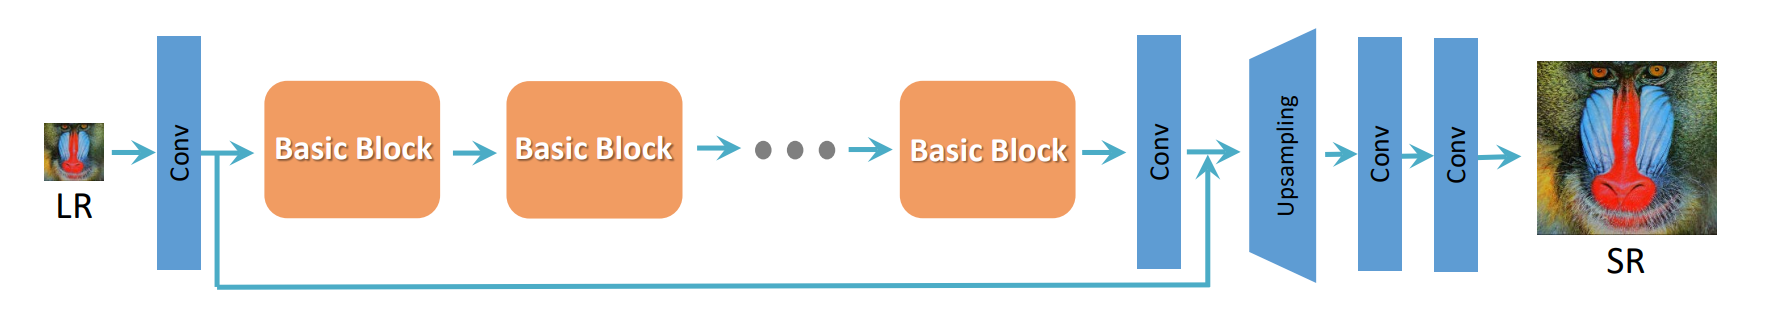
\includegraphics[scale=0.25]{figures/SRResNet.png}
  \caption{The basic architecture of SRResNet.}
  \label{img:SRResNet}
\end{figure}

ESRGAN stands for Enhanced SRGAN and introduces some major improvememnts to the structure of the network. The core structure of the network employs an SRResNet architecture (Figure \ref{img:SRResNet}) with two notable differences: the lack of batch normalization and a new structure that replaces the original basic block with the proposed Residual-in-Residual Dense Block (RRDB), which combines multi-level residual network and dense
connections as depicted in Figure \ref{img:RRDB}

\begin{figure}[H]
  \centering
  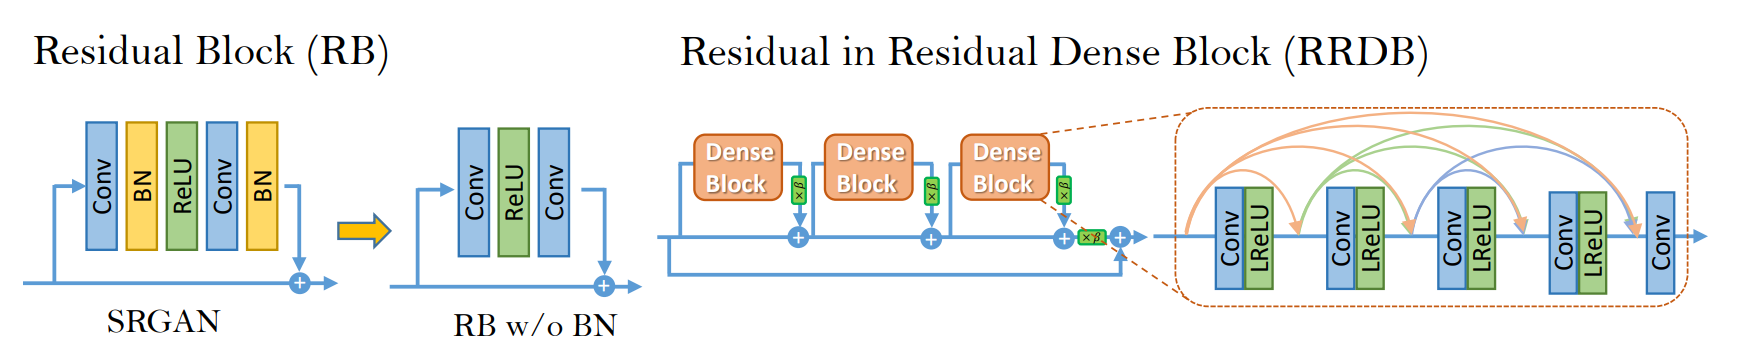
\includegraphics[scale=0.25]{figures/RRDB.png}
  \caption{Left: BN layers removed from residual blocks in SRGAN. Right: RRDB block used in the new deeper model.}
  \label{img:RRDB}
\end{figure}

\subsection{Real-ESRGAN}
\label{subsec:esrgan}

\subsection{HAT-L}
\label{subsec:esrgan}

\subsection{SwinIR}
\label{subsec:esrgan}
